\subsection{Forecasting Algorithms}
We adapt two basic forecasting algorithms from current literature to evaluate the
performance of our expanded vocabularies.
The first model is a naive model, dubbed the
\emph{``unique visitor model"}, adapted from \cite{saez2011total} and \cite{tumasjan2010predicting},
and forecasts elections based on the counts of mentions of a candidate. 
The second model uses a regression fit to map from tweet features to opinion polls and thus forecast elections.
We dub this model as the \emph{``regression model"} and this approach
is adapted from \cite{bermingham2011using} and \cite{o2010tweets}.

\noindent
{\bf Unique Visitor Model:}
The assumption here is that
large parties that are more popular will have a larger social media footprint than smaller and less popular parties. 
Further bot-generated tweets from election campaigns can artifically boost candidate mentions.
This model estimates the relative popularity of candidates contesting the election by accounting for the unique
users tweeting about the candidate and thus aiming to normalize such effects.
The seed vocabulary for PSL is crafted by hand and includes the candidate's names and aliases, the name and acronyms for his/her political party and the official Twitter handle of the candidate.
For the given time period, the tweets from the country in question are tracked for the occurrence of the terms in the vocabulary.
We then build a time series of sentiment (from Lexalytics) and Klout scores (from Klout.com) from the tweets returned.
The absolute popularity of a candidate $C_d$ is calculated as:
\begin{equation}
{C_d} = \sum_{i \in \textrm{Users}} K_i \times UCS_{id}
\end{equation}
\noindent
where $K_i$ is the Klout score for user $i$, and $UCS_{id}$ is User Candidate Score, the average of sentiment scores for all tweets from user $i$ about candidate $d$. These popularities are normalized and used to forecast the relative proportion of votes.

\begin{figure*}
	\centering
	%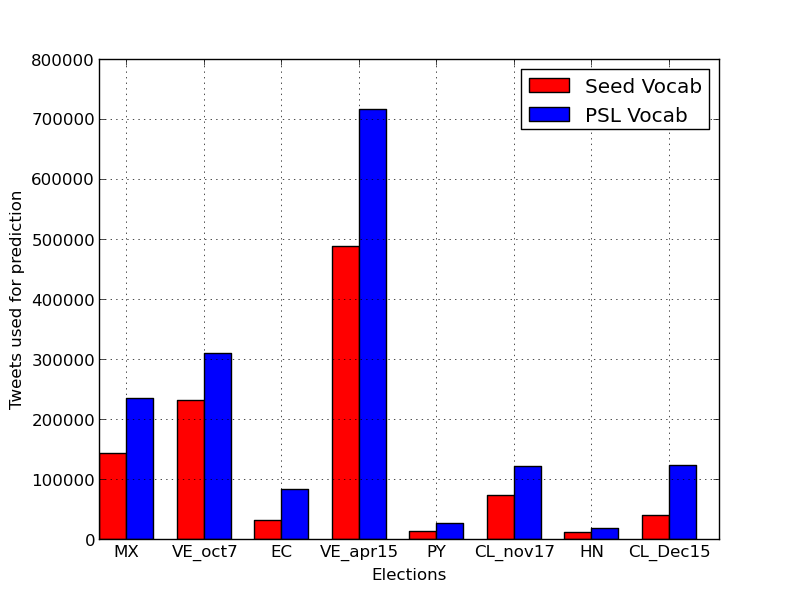
\includegraphics[scale=0.40]{support_files/Recall.png}
	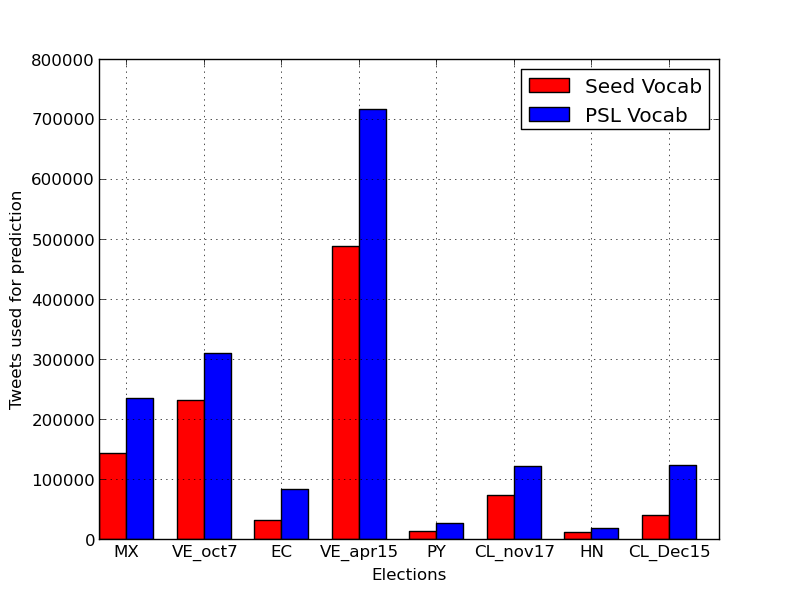
\includegraphics[	height=0.23\textheight, width=0.60\textwidth]{support_files/Recall.png}
	\caption{Retrieval increases using the PSL vocabulary w.r.t. the seed vocabulary.}
	\label{fig:recall}
\end{figure*}

\noindent
{\bf Regression Model:}
In this model, in addition to tweets, we leverage any opinion polls available for the elections 
to make our predictions.
Like the earlier model we track the tweets that mention words/phrases
from the vocabulary defined for each candidate.
We then conduct a linear regression fit that uses the opinion polls as dependent variable and features generated from 
these tweets as independent variable.
We reason that by regressing from the Twitter features to the opinion polls the bias due to Twitter being a non-representative sample
can be mitigated.
We use a total of six features: Klout scores, number of unique users, total number of mentions, sentiment, and incumbency.
The Klout scores, unique users, and mentions are further categorized into positive and negative mentions.
We normalize each of these features across all candidates to obtain the relative share of the volume. 
When there is more than one polling house publishing an opinion poll (for the same date) we take the average of the polls. 
Table~\ref{table:coeff} details the coefficients learned for each feature averaged over all the candidates from all the elections.
The values confirm our hypothesis that the number of unique users and sentiment have more predictive power than total number of mentions.
Intuitively it is also seen that the coefficients for share of negative users and negative mentions carry a negative weight.
Another interesting observation is the fact that the incumbency binary variable is not as predictive which could be
due to a confounding effect with other features. Having learnt a regression fit, we forecast the election
by using features in the 10 day window leading upto the prediction date.

\iffalse
\subsection{Performance}
The Unique Visitor Model and the Regression Model were tested exhaustively on a total of 36 elections from Latin America during 2012 and 2013 ranging from local mayoral elections to presidential elections at the country level.
It is important to note that every single election was predicted ahead of time and not in retrospect.
The tweets were purchased from DataSift, an infoveilence service that resells Twitter data.
On an average we collected close to 2 million unique tweets a day from over 21 countries in Latin America.
Then these tweets were geo-coded using a geo-location algorithm we developed to obtain tweets from the country of interest.
Only tweets from the locations pertaining to elections were used to make the predictions.
For example, for the Rio de Janeiro Mayor elections only tweets from the city of Rio de Janeiro were used and similarly for state level Governor elections only tweets originating from that particular state were used.
Once the tweets were filtered by location the time series of Klout and sentiment scores were calculated by tracking the tweets for the mentions of candidate.

Table~\ref{table:trackRecord} shows the overall performance of the two models. 
It can be noticed that the accuracy drops as the granularity of the elections increases. 
This is primarily due to the fact that opinion polls were available only for the country level elections.
Therefore, we could not use the Regression Model for the state or city level elections.
This increased the error as the predictions were generated only from the naive Unique Visitor Model.
Also, from the tweets collected it was noticed that there wasn't much chatter on Twitter about 
smaller, local, elections.
This skewed the results as the model tracking the names of the candidates was not as accurate as desirable.
If the city level elections were ignored as outliers the overall accuracy of the models improves to 91.6\%.
\fi
